\documentclass[MASTER.tex]{subfiles}
\begin{document}

	
	\begin{frame}
	\Large
		\frametitle{Zero-Inflated Negative Binomial regression}
\begin{itemize}
\item  We are going to use the variables: \textbf{child} and \textbf{camper} to model the count in the part of negative binomial model and the variable \textbf{persons} in the logit part of the model. 
\item We use the \textbf{pscl} to run a zero-inflated negative binomial regression. 
\item We begin by estimating the model (called \texttt{m1}) with the variables of interest.
\end{itemize}	
		

\end{frame}
%============================================================================== %
\begin{frame}[fragile]
	\large
\begin{verbatim}
		
		m1 <- zeroinfl(count ~ child + camper | persons,
			  data = fishing, dist = "negbin", 
			  EM = TRUE)
		
		summary(m1)
\end{verbatim}
\end{frame}
%============================================================================== %
\begin{frame}[fragile]
	\begin{verbatim}
		## Call:
		## zeroinfl(formula = count ~ child + camper | persons, 
		##     data = fishing, 
		##     dist = "negbin", EM = TRUE)
		## 
		## Pearson residuals:
		##    Min     1Q Median     3Q    Max 
		## -0.586 -0.462 -0.389 -0.197 18.013 
\end{verbatim}
\end{frame}
%============================================================================== %
\begin{frame}[fragile]
	
	\begin{itemize}	
		\item Below the model call, you will find a block of output containing negative binomial regression coefficients for each of the variables along with standard errors, z-scores, and p-values for the coefficients. 
		\item A second block follows that corresponds to the inflation model. This includes logit coefficients for predicting excess zeros along with their standard errors, z-scores, and p-values.
	\end{itemize}
\end{frame}
%============================================================================== %
\begin{frame}[fragile]
	\begin{verbatim}
		## Count model coefficients (negbin with log link):
		##             Estimate Std. Error z value Pr(>|z|)    
		## (Intercept)    1.371      0.256    5.35  8.6e-08 ***
		## child         -1.515      0.196   -7.75  9.4e-15 ***
		## camper1        0.879      0.269    3.26   0.0011 ** 
		## Log(theta)    -0.985      0.176   -5.60  2.1e-08 ***
\end{verbatim}
\end{frame}
%============================================================================== %
\begin{frame}[fragile]
	\begin{verbatim}
		## Zero-inflation model coefficients (binomial with logit link):
		##             Estimate Std. Error z value Pr(>|z|)  
		## (Intercept)    1.603      0.836    1.92    0.055 .
		## persons       -1.666      0.679   -2.45    0.014 *
		## ---
		## Signif. codes:  0 '***' 0.001 '**' 0.01 '*' 0.05 '.' 0.1 ' ' 1 
		## 
		## Theta = 0.373 
		## Number of iterations in BFGS optimization: 2 
		## Log-likelihood: -433 on 6 Df
\end{verbatim}
\end{frame}

%============================================================================== %
\begin{frame}[fragile]
\frametitle{Tests of Significance}
\begin{itemize}
\item	All of the predictors in both the count and inflation portions of the model are statistically significant. 
\item This model will fit the data significantly better than the null model, i.e., the intercept-only model. 
\item To show that this is the case, we could compare with the current model to a null model without predictors using chi-squared test on the difference of log likelihoods. 
\end{itemize}	

\end{frame}
%%============================================================================== %
%\begin{frame}[fragile]
%	\begin{verbatim}	
%	
%	m0 <- update(m1, . ~ 1)
%	
%	pchisq(2 * (logLik(m1) - logLik(m0)), df = 3, lower.tail=FALSE)
%	
%	## 'log Lik.' 1.28e-13 (df=6)
%\end{verbatim}
%\end{frame}
%============================================================================== %
%=================================================================================================================== %
\begin{frame}
	\begin{figure}
		\centering
		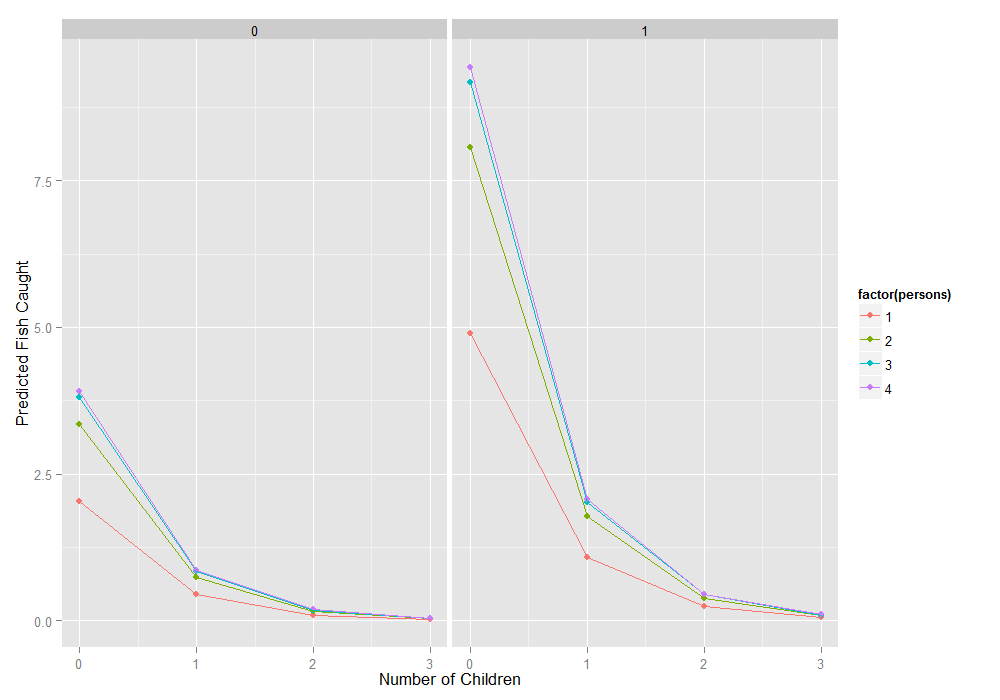
\includegraphics[width=0.7\linewidth]{zinbreg10}
		
	\end{figure}
	
	%newdata1 <- expand.grid(0:3, factor(0:1), 1:4)
	%colnames(newdata1) <- c("child", "camper", "persons")
	%newdata1$phat <- predict(m1, newdata1)
	%
	%ggplot(newdata1, aes(x = child, y = phat, colour = factor(persons))) +
	%  geom_point() +
	%  geom_line() +
	%  facet_wrap(~camper) +
	%  labs(x = "Number of Children", y = "Predicted Fish Caught")
	
\end{frame}
\end{document}	